\documentclass{article}
\usepackage[utf8]{inputenc}
\usepackage{aaai17} %Required
\usepackage{graphicx} %Required
\usepackage{amsmath}
\usepackage{float}
\frenchspacing %Required
\setlength{\pdfpagewidth}{8.5in} %Required
\setlength{\pdfpageheight}{11in} %Required
\begin{document}

\title{A Human-Computation Platform for Multi-Scale Genome Analysis}

%\author{Akash Singh \qquad Chris Drogaris \qquad Jerome Waldispuhl\\McGill University\\author@mail.mcgill.ca
%}

\author{Akash Singh*, Chris Drogaris*, Elena Nazarova, Mathieu Blanchette \and J\'er\^ome Waldisp\"uhl\\ School of Computer Science, McGill University \\ jeromew@cs.mcgill.ca \AND
Anjum Ibna Matin*, Mardel Maduro \and Olivier Tremblay-Savard \\ Department of Computer Science, University of Manitoba \\ tremblao@cs.umanitoba.ca \\ (*equal contribution)}

\maketitle
\begin{abstract}
We introduce a citizen science framework for a collective curation genomic annotation at multiple levels of the genome organisation. Currently our system aims to integrate a fully new version of Phylo solving the Multiple Sequence Alignment (MSA) problem, with a new game aiming to understand the evolution of large scale genomic regions.
%This paper introduces a new version of citizen science game: Phylo to solve Multiple Sequence Alignment (MSA) problem. 
%The new version of Phylo includes alignments based on motif patterns and uses improved metrics based on the results and statistics collected since the game came out in 2012. The new evolution game that we propose tackles the genome sorting 
\end{abstract}
\section{Introduction}
Human computation tasks stream appear in many scientific problems, such as in astronomy \cite{skibba2012galaxy}, molecular biology \cite{cooper2010predicting,kawrykow2012phylo}, neuroscience \cite{kim2014space}, and even quantum physics \cite{lieberoth2015getting}.
% Likewise, in 2010, we released a game-with-a-purpose named
Phylo (\texttt{http://phylo.cs.mcgill.ca}), is a citizen science game which aims to help us improve the accuracy of the comparison of DNA data \cite{kawrykow2012phylo,kwak2013open}. Phylo annotations aim to help geneticists in various tasks such as studying evolution and understanding mutations that cause genetic disorders. First, we present a new design of Phylo which features novel functionalities such as transcription factors annotations, better feedback to users, and enhancements in game metrics based on the observation made on the data collected by Phylo since 2010.
Next, we introduce a new game addressing a different problem in comparative genomics occuring at a higher level of the genomic organization: the genome sorting problem. In the latter, the user aims to find the minimum number of evolutionary events (e.g. duplications, deletions, inversions) needed to transform one genome into the other.

% This paper presents a new design of Phylo which also includes finding similar motif patterns across different species and providing information about its transcription factor. There are major enhancements in the feedback given to the players, as we not only aim to make the game for casual players, but also, making it more informative to educate these players. The game also includes significant changes in terms of its design algorithms and metrics based on our observations of the collected data since 2012.

% Phylo converts MSA problem into small puzzles that can be played by the users either on web or using mobile application (available only for the proposed version in this paper). We convert the multiple alignment problem to a game where the goal is to align words made by cubes of different color instead of letters representing the genetic code (A, C, G, T) and motif patterns are represented as series of diamonds on top of these cubes. The sequences are displayed on a grid where you can only move the cubes horizontally. The goal of the player is to maximize the similarity within a column and reduce the number of gaps. The rest of the paper proposes upgrades in the game design. Our purposes are to (1) show changes in metrics based on our observations of data from Phylo until now, and (2) addition of new functionalities in the upgraded version of Phylo.
\begin{figure}
 \centering
  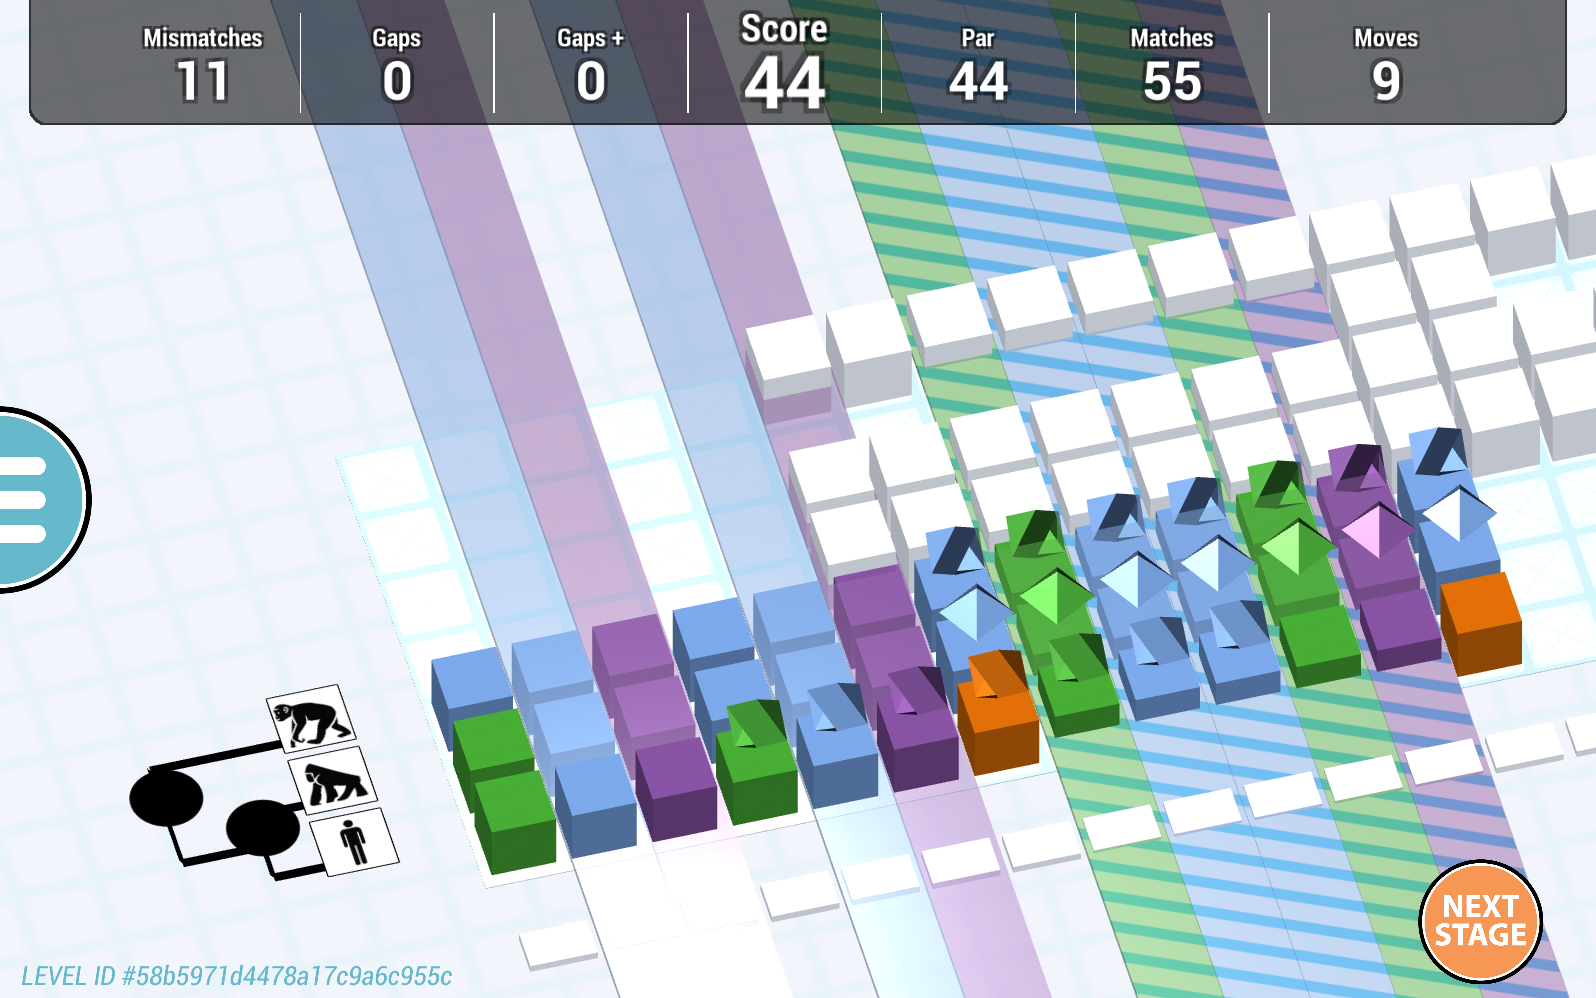
\includegraphics[width=0.5\textwidth]{Phylo3_3.png}
 \caption{Phylo novel interface. Each color of cube represents a nucleotide in DNA sequence. Users can move the bricks horizontally, and try to maximize similarity within a column. The diamonds on top of the cubes indicate the putative presence of a functional motifs.}
 \label{fig:1}
\end{figure}
\section{Phylo}

\subsection{Proposed Methods}
Phylo will still primarily aim to solve the multiple sequence alignment problem, used to reveal conserved DNA sequence across species. In addition, our novel implementation will feature improved design, enhanced portability, and new functionalities.
\begin{enumerate}
  \item \textit{Motif based alignments}: The DNA binding specificity of transcription factors (TF) are generally highly conserved among related organisms.    
% Therefore, DNA binding profiles for human and mouse transcription factors are almost identical, making the information about transcription factor specificity interchangeable between mammalian organisms. 
% This is also true with respect to promoter enriched motifs - vertebrates are generally all enriched for the same promoter motifs (SP1, NFY,etc). However, different sets of organisms, such as fruit flies, or yeast, or plants, or others often contain completely different repertoires of transcription factors and motifs. 
Database of known TF motifs is now maintained in Phylo \cite{heinz2010simple}. But this information is not highly specific. Users are shown with a roster of putative TF motifs present in the puzzle. The alignment of these motifs will allow the users to collect rewards and help us to false positive annotations. 

% They are required to align the blocks based on motifs to earn extra reward/bonus. Extra points or bonus is rewarded if the players are able to align the sequences of other species with an accuracy of 80\% or above. A similarity of 80\% or above in motifs that are unknown to that species can be considered as conserved among species. These motifs are 'unknown' because we do not know the principle factors that bind them. But in most cases, we can consider them as the DNA binding domains for which the TFs are either unknown or for which the data is not really available. Such regions can also be described as being conserved, which is the central idea of motifs.

% These motifs can also play a significant role in finding disease causing mutations. Since we already know from various databases about the presence of similar motifs in a given set of species, we can define the change that causes a disease by comparing the sequences based on these known regions.
  
  \item \textit{Enhanced feedback to players:}   
%   We observed from our phylo data collected since 2012, that there is a significant improvement in players performance when they become an expert (played more than 40 puzzles) when compared to rookies (played less than 20 puzzles). F-test reflects the same with a P-value of  0.018 for difficult puzzles between rookies and experts. 
%   With the inclusion of motifs in phylo database, we have enhanced the feedback to the users by mapping each motif with its transcription factor name, DNA binding domain and its origin (mostly ChIP-Seq data sets). 
%  In addition, w
We now made the game more informative so as to educate the players simultaneously by including the exact disease causing mutation, motif sequences and its annotation in the human gene sequence which will be shown to them once they complete the puzzle.
  \item \textit{Evaluation of users based on their click-stream data}: Our systems will include mechanisms to analyze user tactics through an analysis of click-stream data. This version of Phylo will feature an inbuilt storyline, helping us to introduce advanced concepts to the users.
% * <olivier.tremblay.savard@gmail.com> 2017-06-30T05:43:49.415Z:
% 
% > Human-Computers
% ???
% 
% ^.
%   , we can easily distinguish players who are playing just for fun from those who are also looking into the educational side of it. 
  \item \textit{Transition to RNA:} This version of Phylo will also take a transition for solving MSA of RNA sequences. The massive player count of Phylo will definitely help in enhancing RNA alignments.
  
%   In addition, this information may get stored to analyze the gaming habits of users which can provide opportunities for upsell or cross-sell, and identify profiles of specific kinds of users. Further, different citizen-science games can be refered or advertised to different users based on their profiles, which we believe can help others games-with-a-purpose.
\end{enumerate}
\subsection{Enhancements in Metrics}

% On reviewing the results and user statistics collected since 2012 by our platform Phylo, we observed that 57\% of the user aligned puzzles were either better or at par with the machine aligned sequences. This indicates that although users are not always able to produce improved alignments, they do so in a non-negligible fraction of the puzzles. Therefore, by analyzing the performance of Phylo, we identified not only its success but also its snags.

\begin{enumerate}
  \item \textit{Puzzle Extraction:} The puzzle database is obtained from Ensembl genome browser\cite{aken2016ensembl}. Human genes associated to diseases and their mutations were noted from HGMD\cite{lualdi2017vitro}. Puzzles are extracted using EnsEMBL Compara. Puzzle extraction criteria have also been updated by additional constraints to increase the accuracy of Phylo.
%   by providing the human chromosome number along with the sequence region start and end coordinates. Puzzles were approved if it meets the following criteria: (1) Number of sub-strings of DNA (A,C,G,T) each puzzle should contain is $\dfrac{3}{2}$ of the number of species or sequences in the puzzle, (2) the ratio \(R(Gaps)=\dfrac{n_{gaps}}{(n_n + n_{gaps})} \) of number of gaps ($n_{gaps}$) to the total of number of nucleotides ($n_n$) and number of gaps($n_{gaps}$) should be greater than 0.3 but less than 0.5, and (3) the puzzles is "interesting" which is the ratio \(R(Intresting)=\dfrac{n_{m}}{(n_m + n_{s} +{n_{gaps}})} \) between number of matches ($n_m$) and sum of number of matches($n_m$), mismatches($n_s$) and gaps($n_{gaps}$) is atmost 0.55 to ensure a non-optimal region. The size of the puzzle is kept dynamic to ensure any change in game interface.
  \item \textit{Puzzle Difficulty:} Difficulty level of puzzles is important in order to route it to its correct difficulty in the game and also routing it based on the players skill level. 
%   Instead of giving the difficulty of puzzle based on number of sequences present in a puzzle, 
We now propose to use the neural network regression model using a vector of 11 features:
% whose hyper parameter values with L2-norm regularization (weight of $10^{-3}$) and 300 nodes in each of the two hidden layers. In order to train a machine learning predictor to recognize difficulty of puzzles, these puzzles need to be represented using a vector of 11 features:
% We extracted and evaluated the following 11 features calculated from the machine-computed MSA: 
(1-4) proportions of $A$, $C$, $G$, and $T$ in $S$, (5) proportion of gaps, 
(6) mean $GC$ content (this relates to the structural properties of DNA), (7) mean entropy of alignment columns, 
(8) average length of sequences, 
(9) number of sequences, 
(10) tree-entropy, and
(11) score of machine-computed alignment.

% The difficulty obtained for puzzles using this model has an accuracy of 72\%.
%   \item \textit{Puzzle Scoring:} The scores for puzzles are evaluated using an affine gap cost model. To give a comparative analysis, the new scheme uses integer values (the score for a match is +1, for a mismatch -1, for a gap opening -4 and for a gap extension -1), which approximate those used by BLASTZ\cite{schwartz2003human}. Motifs are scored using the probability matrix. The scores are calculated by adding the log-odds probabilities for the nucleotide found in each position\cite{heinz2010simple}. Players get a bonus equivalent to the motif score for aligning the sequences similar to the motif pattern (at least 80\%), for each species which meets this criteria. This bonus is added to the original score and get help them better rankings against those who align the sequences without motifs. This change allows gamers to make a transition from solving MSA to motif based sequence alignments.
\end{enumerate}

\section{Evolution Game}

\subsection{Genome Sorting Problem}

Similarly to the MSA problem, the genome sorting problem has received a lot of attention from the comparative genomics community in the last decades. Given two genomes (represented by gene orders), the goal is to find the shortest sequence of biological events to transform one genome into the other. When both genomes have exactly one copy of each gene, the problem is simpler. For example, in this context (one copy of each gene), sorting genomes by reversals (inversions of segments of genes) can be solved in polynomial time~\cite{hannenhalli1999transforming,tannier2007advances}.
However, it is often the case that genomes have multiple copies of certain genes. In this case, the genome sorting problem becomes NP-hard in the case of sorting by reversals~\cite{christie2001sorting}, or sorting by reversals and duplications~\cite{chen2005assignment} for example.

\subsection{Objectives}

As a first step towards the development of new algorithmic methods to study genome evolution in highly divergent genomes with duplicate genes, our goal is to develop a new crowdsourcing and human computing game that will ask players to find optimal evolutionary scenarios transforming one genome into another. Our game takes the form of a puzzle game and will be targeting both casual players and biology students, just like Phylo. In addition to obtaining optimal evolutionary scenarios from the players, we will record every move that the players make. This will allow us to analyze the strategies employed by the players to solve those problems, and this information will then be used as inspiration to develop new algorithmic methods.

\subsection{Input Data and Possible Events}

Our game will first focus on sorting bacterial genomes, which are simpler because they have only one chromosome. 
The list of possible evolutionary events (i.e. available player moves) will be the three types of events that are mostly observed in bacterial genomes: duplications of genes, deletions of genes, and inversions of segments of genes. Bacterial genomes also have an interesting characteristic: inversion events occur mostly around the terminus of replication, which is located approximately in the middle of the genome. Consequently, only inversion events of segments of genes that are overlapping the terminus will be considered as valid moves.

\begin{figure}
 \centering
  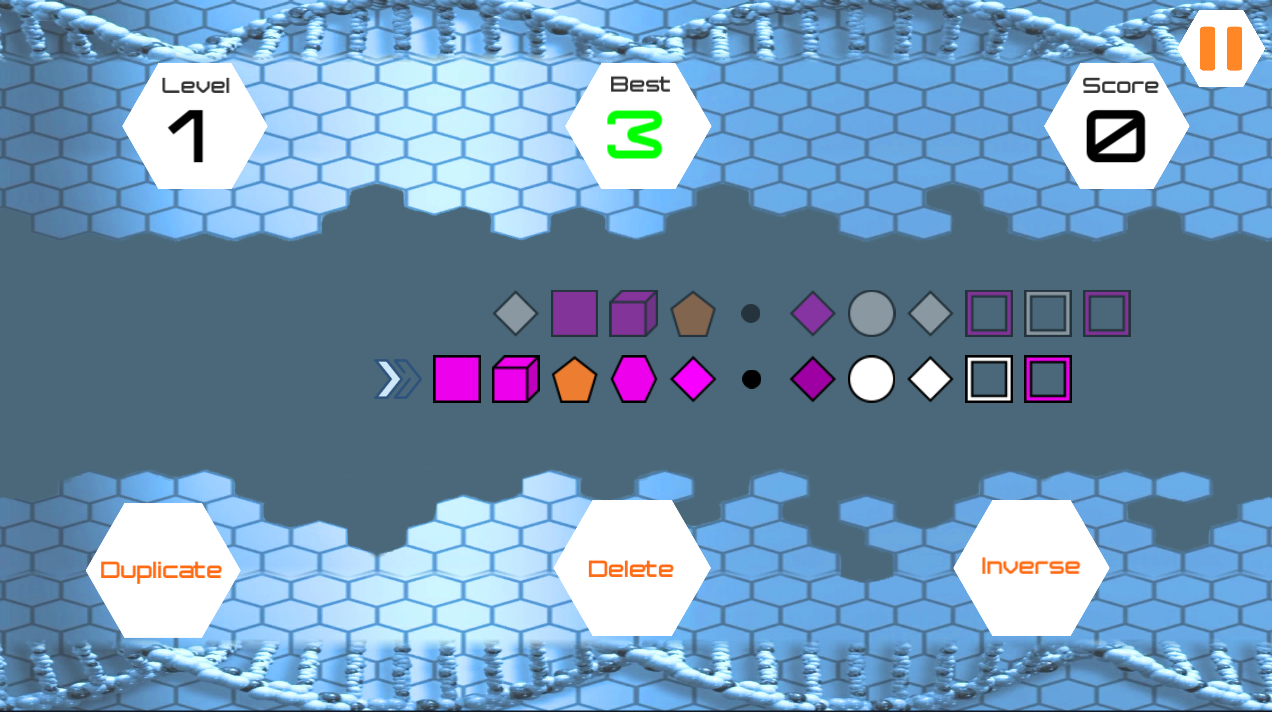
\includegraphics[width=0.48\textwidth]{EvoGame.png}
 \caption{Evolution Game interface. Each colored shape represents one gene and the black dot in the middle represents the terminus of replication. The top genome is the target: players have to apply evolutionary events to the bottom sequence to transform it into the target.}
 \label{fig:2}
\end{figure}
\subsection{Interface}

The interface of the Evolution Game is shown in Figure~\ref{fig:2}. At the very top of the screen, information on the level, best score (out of all the other players for this level) and the current score of the player is shown. The player's score on a level is simply the total number of evolutionary events that was used up to this point. The middle part of the screen shows the two genomes, represented as sequences of colored shapes (i.e. genes). The top genome is the target, whereas the bottom one is the mutable genome. Finally, the bottom panel has three buttons, which correspond to the three possible evolutionary events. In order to apply one of these events, the player has to select the genes of the mutable sequence that will be modified, and then click on the event type. In the case of a duplication, there is one last step after clicking the duplicate button: select where the genes will be duplicated in the genome. Once both genomes are identical, the player will be prompted to continue to the next level, or to restart the level if the player wants to improve his/her score.

\bibliographystyle{aaai}
\bibliography{Bib.bib}
\end{document}
